\section{QEMU下SD卡的驱动理解}
本节介绍在非实物环境下,使⽤qemu模拟SD卡块设备条件下的SD卡驱动。在qemu环境下,块设备驱动程序主要依赖virtio,本节介绍virtio标准相关内容及virtio下host和guest之间设备数据交互过程,最后使⽤实现该标准的第三⽅依赖库介绍npucore中QEMU下块设备驱动的实现。
随着互联网和云计算的兴起,物理服务器上通过虚拟机技术运行多个虚拟机,并在虚拟机中运⾏guest操作系统的模式成为主流。在传统的全虚拟化解决⽅案中,guest OS要使⽤host 资源,需要Hypervisior来截获所有的请求指令,然后模拟出这些指令的⾏为,半虚拟化通过底层硬件辅助的⽅式,将部分没必要虚拟化的指令通过硬件来完成,Hypervisor只负责完成部分指令的虚拟化,guest完成不同设备的前端驱动程序,Hypervisior配合guest完成相应的后端驱动程序,两者之间通过某种交互机制实现虚拟化过程。由于不同guest前端设备其⼯作逻辑⼤同⼩异,单独为每个设备定义⼀套接⼝实属没有必要,⽽且还要考虑扩平台的兼容性问题,另外,不同后端 Hypervisor 的实现⽅式也⼤同⼩异(如KVM、Xen等)。所以,需要⼀套通⽤框架和标准接⼝(协议)来完成两者之间的交互过程。
《virtio: towards a de-facto standard for virtual I/O devices》⾸次提出了Virtio半虚拟化Io模型,它是⼀套通⽤ I/O 设备虚拟化的程序,是对半虚拟化 Hypervisor 中的⼀组通⽤ I/O 设备的抽象。提供了⼀套上层应⽤与各 Hypervisor 虚拟化设备(KVM,Xen,VMware等)之间的通信框架和编程接⼝,减少跨平台所带来的兼容性问题,大大提⾼驱动程序开发效率。

6.3.1 virtio架构

VirtIO由 Rusty Russell 开发,对准虚拟化 hypervisor 中的一组通用模拟设备IO的抽象。Virtio是一种前后端架构,包括前端驱动(Guest内部)、后端设备(QEMU设备)、传输协议(vring)。框架如下图所示:

 
\begin{figure}[H]
    \centering
    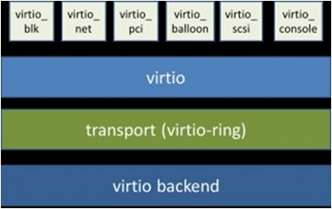
\includegraphics{figures/06-03-1.png}
\end{figure}
前端驱动:

虚拟机内部的 virtio模拟设备对应的驱动。作用为 接收用户态的请求,然后按照传输协议对请求进行封装,再写I/O操作,发送通知到QEMU后端设备。

后端设备:

在QEMU中创建,用来接收前端驱动发送的I/O请求,然后按照传输协议进行解析,在对物理设备进行操作,之后通过终端机制通知前端设备。

传输协议:

使用virtio队列(virtio queue,virtqueue)完成。设备有若干个队列,每个队列处理不同的数据传输(如virtio-balloon包含ivq、dvq、svq三个)。

virtqueue通过vring实现。Vring是虚拟机和QEMU之间共享的一段环形缓冲区,QEMU和前端设备都可以从vring中读取数据和放入数据。

QEMU如何感知虚拟机的操作的?虚拟机内调用kick函数实现通知之后,会产生KVM_EXIT。Host端的kvm模块捕获到这个EXIT之后,根据它退出的原因来做处理。如果是一个IO_EXIT,kvm会将这个退出交给用户态的QEMU程序来完成IO操作。

QEMU为kvm虚拟机模拟了virtio设备,因此后端的virtio-pci设备也是在QEMU进程中模拟生成的。QEMU对模拟的PCI设备的配置空间注册了回调函数,当虚拟机产生IO_EXIT,就调用这些函数来处理事件。

virtio设备通过特定于总线的⽅法发现和识别,每个设备由以下⼏个要素组成:

(1)设备状态字:设备状态字指⽰了在驱动程序初始化设备期间的设备状态,定义以下⼏个状态:

ACKNOWLEDGE(0x0000001):guest OS已找到设备,并将其识别为有效的virtio设备。

DRIVER(0x00000010):guest OS知道如何驱动设备

FAILED(0x10000000):设备出现问题。

FEATURES_OK(0x00000100):指⽰驱动程序以取⼈其所有功能

DRIVER_OK(0x00000100):指⽰驱动程序已设置并准备好驱动

DEVICE_NEEDS_RESET(0x01000000):指⽰设备需要重启。

(2)特征位:特征位⽤于表⽰virtio设备具有的各种特性和功能,其中bit0 – 23是特定设备可以使⽤的feature bits, bit24 – 37预给队列和feature协商机制,bit38以上保留给未来其他⽤途。驱动程序与设备对设备特性进⾏协商,形成⼀致的共识,这样才能正确的管理设备。

(3)通知:通知是指设备和驱动程序必须通知对⽅,它们有数据需要对⽅处理,有三种类型的通知:配置更改通知,设备->驱动程序,指⽰设备配置空间已更改;可⽤缓冲区通知,驱动程序->设备,指⽰缓冲区可⽤;已使⽤缓冲区通知,设备->驱动程序,指⽰缓冲区已经使⽤。

(4)设备配置空间:设备配置空间通常⽤于配置不常变动的设备参数(属性),或者初始化阶段需要设置的设备参数。设备的特征位中包含表⽰配置空间是否存在的bit位,并可通过在特征位的末尾添加新的bit位来扩展配置空间。设备驱动程序在初始化virtio设备时,需要根据virtio设备的特征位和配置空间来了解设备的特征,并对设备进⾏初始化。

(5)virtqueue虚拟队列

在virtio设备上进⾏批量数据传输的机制被称为虚拟队列(virtqueue),每个设备可以有零个或多个虚拟队列。设备驱动程序向该队列中添加缓冲区描述符并向设备发送可⽤缓冲区通知,通知设备从队列中读取请求;设备处理完请求后将使⽤的缓冲区标记为已使⽤并添加到队列中,向设备驱动程序发送已⽤缓冲区同通知,设备驱动程序从已⽤缓冲区中读取数据。

6.3.2 virtio块驱动整体流程

从代码上看,virtio的代码主要分两个部分:QEMU和内核驱动程序。Virtio设备的模拟就是通过QEMU完成的,QEMU代码在虚拟机启动之前,创建虚拟设备。虚拟机启动后检测到设备,调用内核的virtio设备驱动程序来加载这个virtio设备。

对于KVM虚拟机,都是通过QEMU这个用户空间程序创建的,每个KVM虚拟机都是一个QEMU进程,虚拟机的virtio设备是QEMU进程模拟的,虚拟机的内存也是从QEMU进程的地址空间内分配的。

VRING是由虚拟机virtio设备驱动创建的用于数据传输的共享内存,QEMU进程通过这块共享内存获取前端设备递交的IO请求。

如下图所示,虚拟机IO请求的整个流程:

\begin{figure}[H]
    \centering
    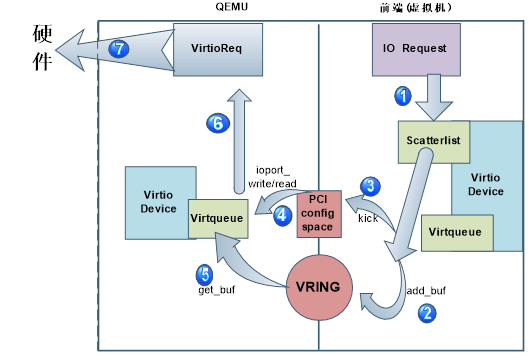
\includegraphics{figures/06-03-2.png}
\end{figure}
1)虚拟机产生的IO请求会被前端的virtio设备接收,并存放在virtio设备散列表scatterlist里;

2)Virtio设备的virtqueue提供add_buf将散列表中的数据映射至前后端数据共享区域Vring中;

3)Virtqueue通过kick函数来通知后端qemu进程。Kick通过写pci配置空间的寄存器产生kvm_exit;

4)Qemu端注册ioport_write/read函数监听PCI配置空间的改变,获取前端的通知消息;

5)Qemu端维护的virtqueue队列从数据共享区vring中获取数据

6)Qemu将数据封装成virtioreq;

7)Qemu进程将请求发送至硬件层。

前后端主要通过PCI配置空间的寄存器完成前后端的通信,而IO请求的数据地址则存在vring中,并通过共享vring这个区域来实现IO请求数据的共享。

从上图中可以看到,Virtio设备的驱动分为前端与后端:前端是虚拟机的设备驱动程序,后端是host上的QEMU用户态程序。为了实现虚拟机中的IO请求从前端设备驱动传递到后端QEMU进程中,Virtio框架提供了两个核心机制:前后端消息通知机制和数据共享机制。

消息通知机制,前端驱动设备产生IO请求后,可以通知后端QEMU进程去获取这些IO请求,递交给硬件。

数据共享机制,前端驱动设备在虚拟机内申请一块内存区域,将这个内存区域共享给后端QEMU进程,前端的IO请求数据就放入这块共享内存区域,QEMU接收到通知消息后,直接从共享内存取数据。由于KVM虚拟机就是一个QEMU进程,虚拟机的内存都是QEMU申请和分配的,属于QEMU进程的线性地址的一部分,因此虚拟机只需将这块内存共享区域的地址传递给QEMU进程,QEMU就能直接从共享区域存取数据。下图为数据共享机制可视化图。
\begin{figure}[H]
    \centering
    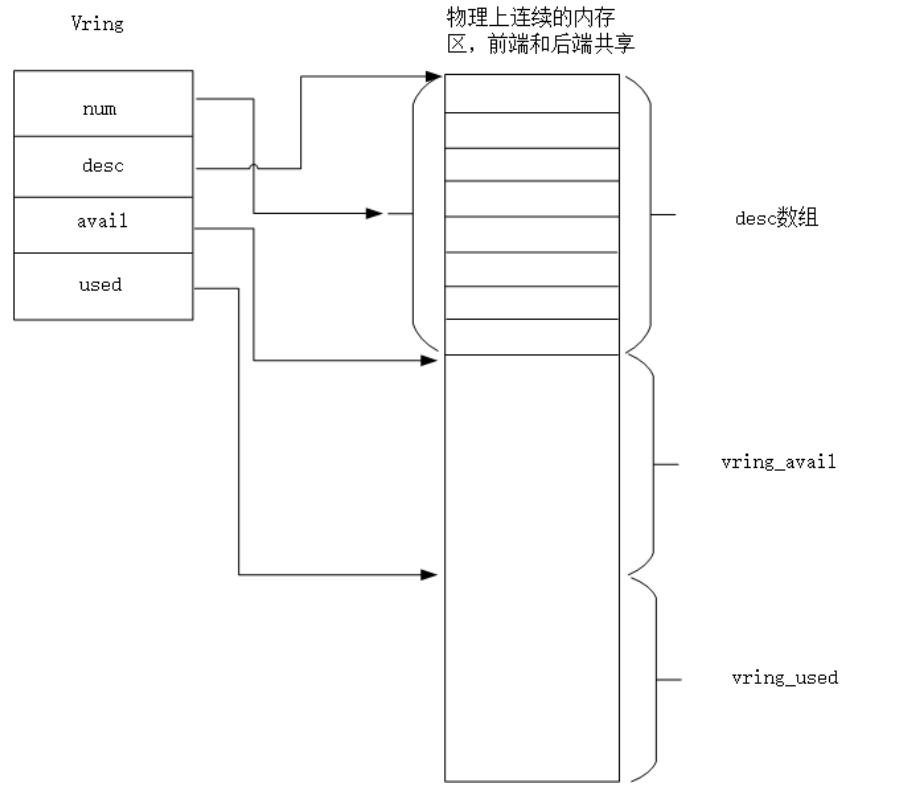
\includegraphics{figures/06-03-3.png}
\end{figure}